 %----------------------------------------------------------------------------------------
%	PACKAGES AND DOCUMENT CONFIGURATIONS
%----------------------------------------------------------------------------------------
\documentclass[11pt]{article}
\usepackage{amsmath} % Required for some math elements
\usepackage{hyperref} 
\usepackage{xcolor}
\usepackage{lipsum} 
\usepackage{cite}
\usepackage{graphicx} % Required for the inclusion of images
\usepackage{algorithmic}
\usepackage{array}
\usepackage{bookmark}
\usepackage{listings}
\usepackage{amssymb}
\usepackage{enumitem}
\usepackage{pythonhighlight}
\usepackage[T1]{fontenc}
\usepackage{inconsolata}
\usepackage[margin=16mm]{geometry}
\usepackage[caption=false, font=footnotesize]{subfig} 

\newlist{steps}{enumerate}{1}
\setlist[steps, 1]{label = Step \arabic*:}

\hypersetup{ %color attributes of citation, link, etc.
    colorlinks=true,
    linkcolor=blue,
    filecolor=gray,      
    urlcolor=blue,
    citecolor=blue,
}

\newcommand{\matlab}{\textsc{Matlab }} %very important and totally necessary addition
\newcommand{\hdotrule}[1]{\hbox to \textwidth{\leaders\hbox to #1pt{\hss . \hss}\hfil}}

\newcommand\Item[1][]{%
  \ifx\relax#1\relax  \item \else \item[#1] \fi
  \abovedisplayskip=0pt\abovedisplayshortskip=0pt~\vspace*{-\baselineskip}}
%----------------------------------------------------------------------------------------
%	DOCUMENT INFORMATION
%----------------------------------------------------------------------------------------

%Here is a little bit of guidance for the report, it should follow this basic structure, or at least cover the topics mentioned here (if you have a different structure in mind). I would expect the report to be < 10 pages, but as there has been no page limit discussed before now, there will be no marks associated with length.

\title{ECEN 405 - Project Report \\ D-Class Sub-woofer Amplifier}
\author{Daniel Eisen : 300447549}
\date{\today}

\begin{document}
\maketitle

\section{Introduction}
 
\textit{Cover the motivation for using a class D in the real world and how it relates to content from ECEN405.}

\newpage
\section{Design}
 
\textit{Here you should describe how your class D amplifier works, giving details of each subsection.
In detail, you should describe the section you designed and the design choices you made. If your team broke up the design of the amplifier in a way that doesn’t suit individual parts being discussed, you will need to talk about the whole design in a bit more detail but you should also describe how the work was delegated and why.}
 
\begin{figure}[h!]
  \centering
  \frame{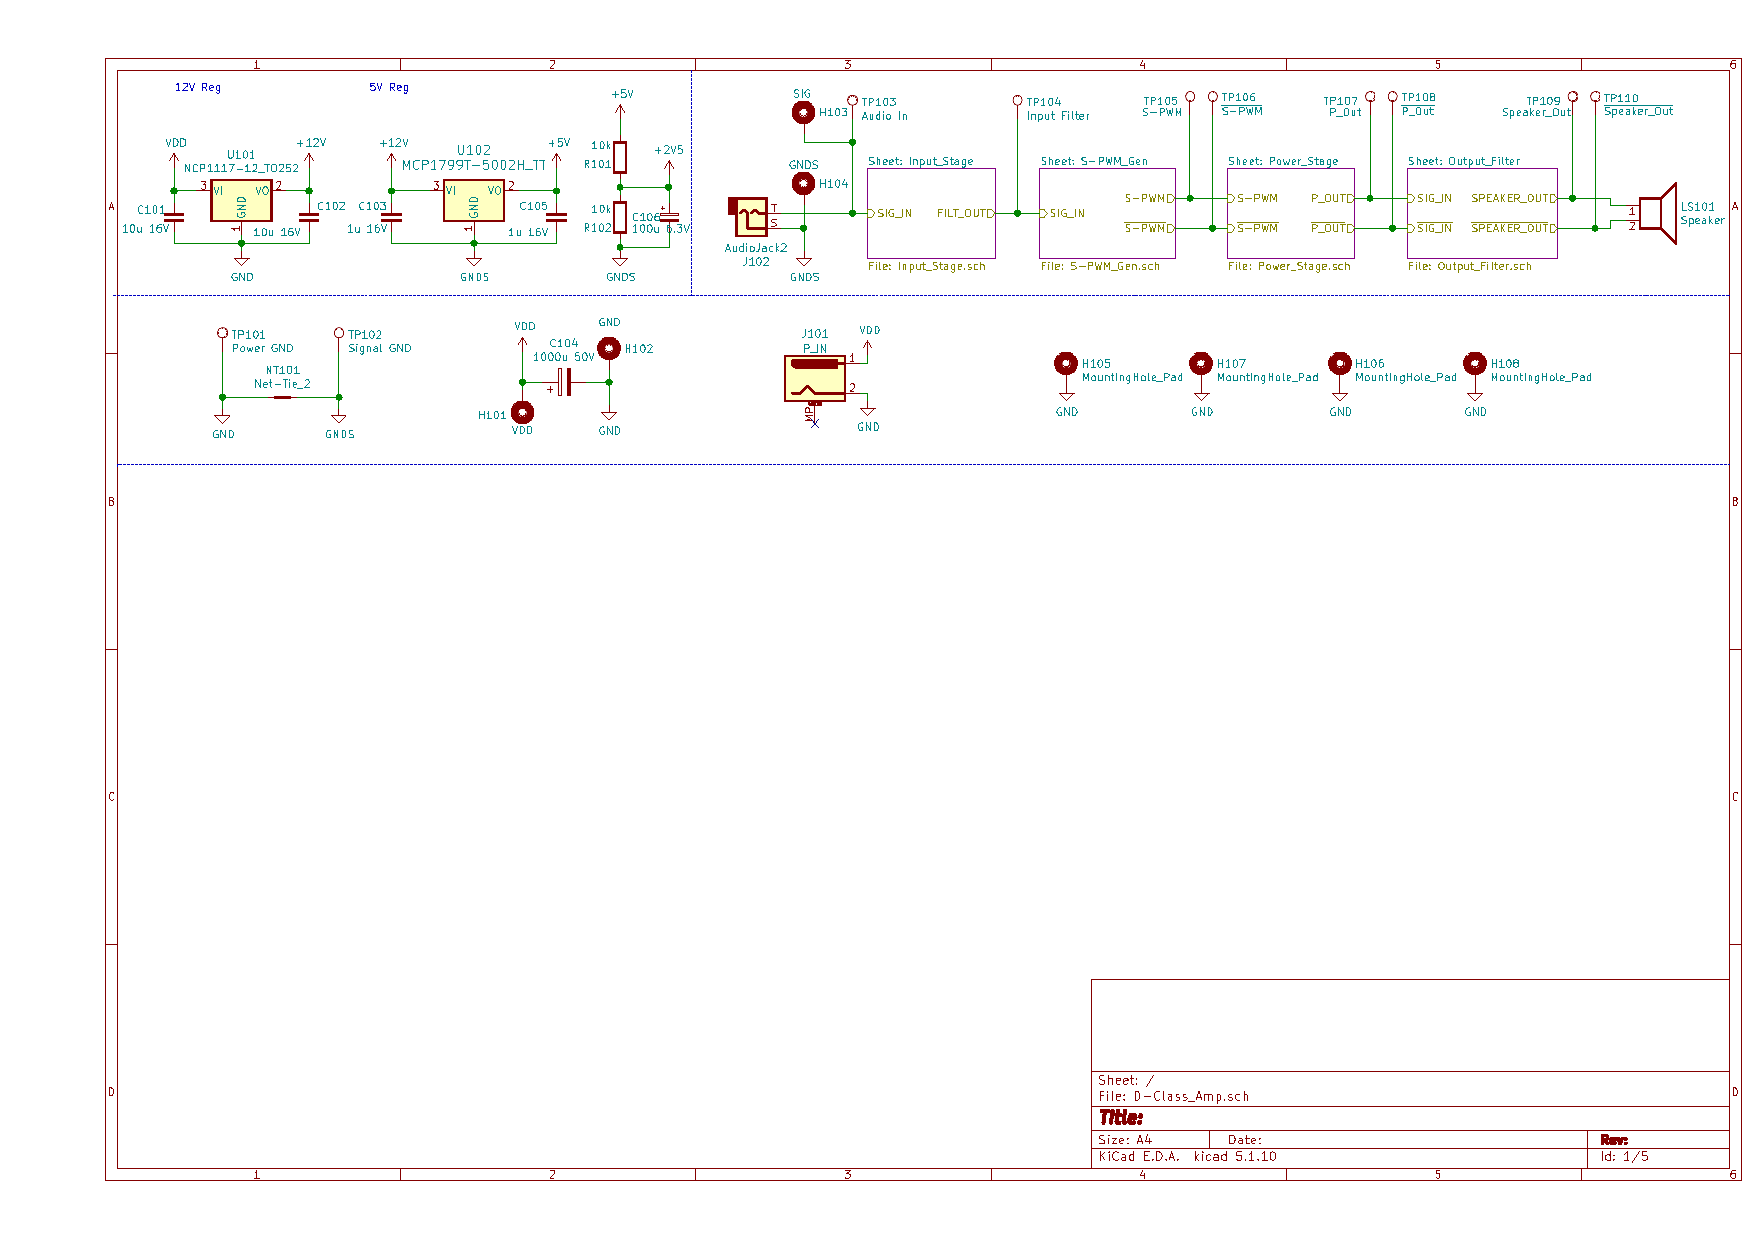
\includegraphics[page=1, trim={18mm 132mm 2mm 10mm},clip,width=0.85\textwidth]{img/schematic.pdf}}
  \caption{High level design schematic}
\end{figure}

\begin{figure}[h!]
  \centering
  \frame{\includegraphics[page=2, trim={25mm 70mm 90mm 60mm},clip,width=0.85\textwidth]{img/schematic.pdf}}
  \caption{Input filtering schematic}
\end{figure}

\begin{figure}[h!]
  \centering
  \frame{\includegraphics[page=3, trim={35mm 133.5mm 30mm 15mm},clip,width=0.85\textwidth]{img/schematic.pdf}}
  \caption{Sampling triangle wave \& SPWM generation schematic}
\end{figure}

\begin{figure}[h!]
  \centering
  \frame{\includegraphics[page=5, trim={85mm 149mm 5mm 12mm},clip,width=0.85\textwidth]{img/schematic.pdf}}
  \caption{Gate driver schematic}
\end{figure}

\begin{figure}[h!]
  \centering
  \frame{\includegraphics[page=4, trim={115mm 97mm 105mm 75mm},clip,width=0.6\textwidth]{img/schematic.pdf}}
  \caption{Output filter schematic}
\end{figure}

\begin{figure}[h!]
  \centering
  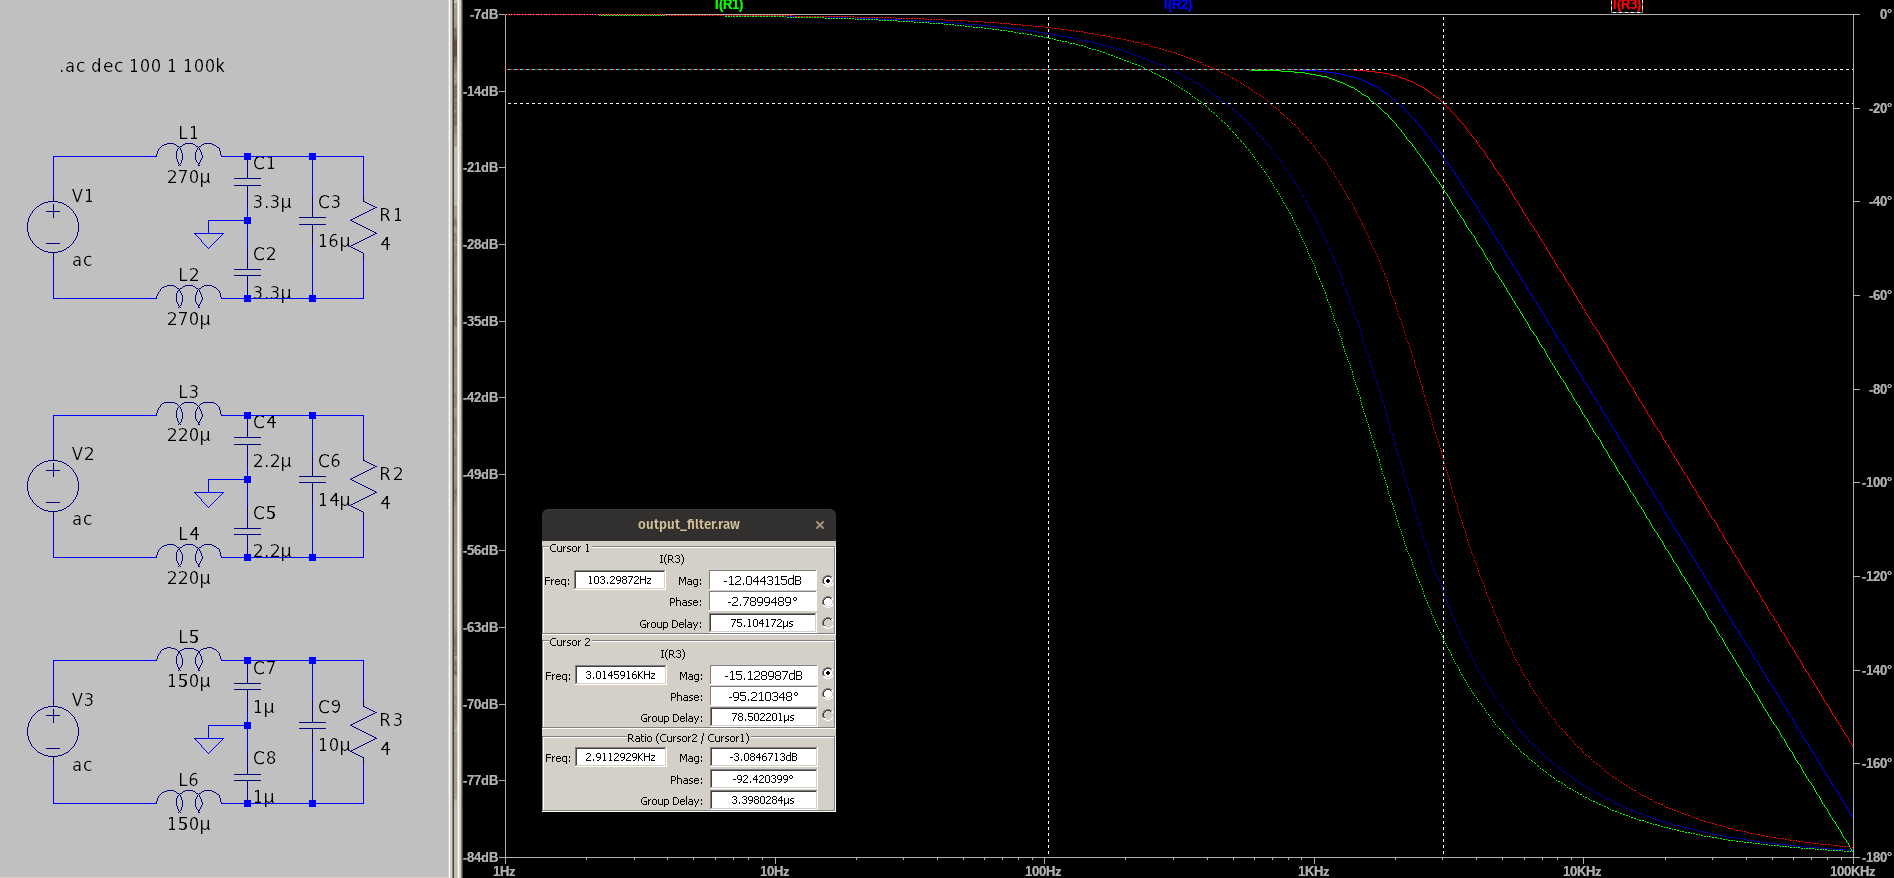
\includegraphics[width=0.75\textwidth]{img/output_filter_sim.png}
  \caption{Output Filter Option Simulations}
\end{figure}


\newpage
\section{Implementation}
 
\textit{Here you should discuss the assembly of the amplifier and any problems you faced as a team building the amplifier.
Here, the individual components should also be characterised. For example: if you have a filter, what is the response and how does it compare to the calculated? If you have a triangle wave, how does it look? Is it doing what I should? Why? Why not? How do the inputs/outputs of your comparator look? How does the square wave on the gate of the MOSFETs look?}
 
\newpage
\section{Results}
 
\textit{Here I would expect to see the results of the whole amp, for example: an output wave, analysis of the efficiency, discuss maximum power output (which may be frequency dependent), and THD.} 
 
\newpage
\section{Conclusions}
 
\textit{What worked, didn’t work? How would you change your approach? Any interesting insights?}
 
\end{document}